\documentclass{pre-tfg}

\usepackage{listings}
\usepackage{formular}
\usepackage[pdftex]{graphicx}
\usepackage{hyperref}
\usepackage{todonotes}

\showhelp  % comenta o borra para eliminar ayudas

\title{(TITLE)}
\author{María González Gutiérrez}
\docdate{(MONTH)}{(YEAR)}


\DeclareGraphicsExtensions{.pdf,.png,.jpg}

\usepackage{color}
\definecolor{gray97}{gray}{.97}
\definecolor{gray75}{gray}{.75}
\definecolor{gray45}{gray}{.45}

\lstset{ frame=Ltb,
     framerule=0pt,
     aboveskip=0.5cm,
     framextopmargin=3pt,
     framexbottommargin=3pt,
     framexleftmargin=0.4cm,
     framesep=0pt,
     rulesep=.4pt,
     backgroundcolor=\color{gray97},
     rulesepcolor=\color{black},
     %
     stringstyle=\ttfamily,
     showstringspaces = false,
     basicstyle=\small\ttfamily,
     commentstyle=\color{gray45},
     keywordstyle=\bfseries,
     %
     numbers=left,
     numbersep=15pt,
     numberstyle=\tiny,
     numberfirstline = false,
     breaklines=true,
   }

% minimizar fragmentado de listados
\lstnewenvironment{listing}[1][]
   {\lstset{#1}\pagebreak[0]}{\pagebreak[0]}

\lstdefinestyle{consola}
   {basicstyle=\scriptsize\bf\ttfamily,
    backgroundcolor=\color{gray75},
   }

\lstdefinestyle{C}
   {language=C,
   }


\renewcommand*\lstlistingname{Listado}



\begin{document}

\maketitle
\tableofcontents

\newpage

El trabajo recogería los siguientes apartados:

\begin{itemize}
\item Introducción (muy recomendable aunque no obligatorio)
\item Tecnología específica cursada por el alumno
\item Objetivos
\item IRÁN TANTAS SECCIONES CENTRALES COMO EL ALUMNO CONSIDERE
\item Medios que se pretenden utilizar
\item Bibliografía básica consultada en la elaboración del anteproyecto
\item Contrato de propiedad intelectual (si lo hubiera)
\end{itemize}


\section{INTRODUCCIÓN}

El capítulo de introducción podrá abordar los siguientes aspectos:

\begin{itemize}
\item Introducción al tema, entorno en el que el trabajo desempeñará
  su objetivo, justificación de la importancia del trabajo abordado.
\item Motivación y antecedentes (con algunas referencias bibliográficas).
\item Descripción gráfica del proyecto (es aconsejable incorporar una figura que describa
  el trabajo a desarrollar y que mejore la comprensión del mismo).
\end{itemize}

Este trabajo fin de grado consiste en un sistema de análisis de texto. El programa procesa un conjunto de textos y extrae una ontología con los personajes, sucesos y relaciones relevantes entre ellos.
Los textos escogidos son del género conocido como \textit{fanfiction}, que se caracteriza por no ser originales: son textos de ficción basados en historias ya existentes, normalmente escritos for fans de la obra original que quieren explorar su mundo y personajes. Para este trabajo se ha escogido un conjunto de \todo{cantidad} \textit{fanfics} basados en \textit{Good Omens} (1990, Terry Prattchet y Neil Gaiman), de modo que se garantiza que tengan personajes, eventos, temas  y tramas en común. El sitio web del que se han extraído los textos es \href{https://archiveofourown.org}{Archive Of Our Own} (AO3 de ahora en adelante), puesto que es el mayor archivo virtual de \textit{fanfics} que existen en internet y permiten la descarga gratuita de todas las obras publicadas en él.

AO3 es un sitio web que reúne a fans de

 El objetivo del proyecto es conseguir una ontología que 

\section{TECNOLOGÍA ESPECÍFICA / INTENSIFICACIÓN / ITINERARIO CURSADO POR EL ALUMNO}

El Trabajo Fin de Grado (TFG, de ahora en adelante) siempre deberá demostrar la aplicación
de las competencias generales de la titulación. Además, el TFG deberá aplicar
\textbf{algunas} de las competencias específicas asociadas a la \textbf{Tecnología
  Específica o Intensificación} que el alumno ha cursado. Por lo tanto, el alumno incluirá
en el anteproyecto \textbf{dos tablas}. Una tabla para seleccionar la tecnología cursada y
en la que se contextualiza el TFG:

\begin{table}[hp]
  \centering
  \caption{Tecnología Específica cursada por el alumno}
  \label{tab:tec-especifica}

  \zebrarows{1}
  \begin{tabular}{p{0.6\textwidth}}
    \textbf{Marcar la tecnología cursada} \\
    \hline
    Tecnologías de la Información \\
    Computación \\
    Ingeniería del Software \\
    Ingeniería de Computadores \\
    \hline
  \end{tabular}
\end{table}


\clearpage

En la segunda tabla, el alumno deberá justificar cómo \textbf{algunas}
de las competencias específicas de la intensificación se aplicarán o
tomarán forma en el TFG, \textbf{La relación de competencias por
  intensificación se encuentran en el Anexo I al final de este
  documento. }


\begin{table}[hp]
  \centering
  \caption{Justificación de las competencias específicas abordadas en el TFG}
  \label{tab:competencias}

  \zebrarows{1}
  \begin{tabular}{p{0.2\linewidth}p{0.7\linewidth}}
    \textbf{Competencia} & \textbf{Justificación} \\
    \hline
    Competencia 1 & [Exponer y argumentar cómo y en qué parte se va a
    abordar esta competencia en el TFG]\\
    & \\
    & \\
    & \\
    \hline
  \end{tabular}
\end{table}


\section{OBJETIVOS}

De acuerdo a la Introducción, el alumno deberá especificar cuál o cuáles son las hipótesis
de trabajo de las que se parten, qué se pretende resolver, y en base a eso formular el
objetivo principal del TFG.

El objetivo principal deberá desglosarse en sub-objetivos parciales. Los sub-objetivos
deberán describirse de forma breve y concisa.

Como preámbulo a la formulación del objetivo parcial, el alumno deberá discutir sobre las
limitaciones y condicionantes a tener en cuenta en el desarrollo del TFG (lenguaje de
desarrollo, equipos, madurez de la tecnología, etc.).

Del mismo modo, será recomendable incluir una lista preliminar de requisitos del sistema a
construir.


\section{RECOMENDACIONES}

Aquí habría que insertar tantas secciones como el alumno considere.

A continuación se indican una serie de recomendaciones que seguidas mejorarán la calificación final del trabajo.

\begin{itemize}
 \item Agrupar párrafos. La división del texto en múltiples párrafos independientes de pequeña longitud dificulta la lectura continua del documento.
\item  Evitar abusar de las listas con viñetas y las enumeraciones.
\item Utilizar un máximo nivel de profundidad secciones de 3 (hasta 3.1.1). Si se hace necesario una división más baja, no hacerlo con enumeración de subsecciones sino con texto en negrita y/o subrayada que represente el comienzo de cada subsección. 
\item  Si no hay más de una sección en un nivel no crearla. Es decir, si no hay al menos una 3.2 no crear la 3.1, ya que no tendría sentido dividir la sección 3.
\item  Utilizar referencias absolutas numéricas a tablas, figuras, secciones, etc. Por ejemplo: en la "Figura 3, se muestra el gráfico que  ..."; "Los resultados finales se encuentran en la Tabla X". Usar los ref y labels para que se actualicen las numeraciones automáticamente. No se debe hablar de ``en la siguiente figura'', ¿Qué pasa si reordeamos el texto o lo hace látex de manera automática?.
\item Cuando se referencia a una tabla, figura, sección, etc. hacerlo con la primera letra en mayúscula, ``En la Sección 1 ...''
\item  El texto siempre debe tener una alineación justificada. 
\item En el inicio de cada sección se debe hacer una breve introducción de lo que contiene y al final, unas pequeñas conclusiones y si es posible un texto de pequeña longitud que una con el siguiente capítulo.
\end{itemize}


\subsection{Inserción de Imágenes}

\begin{figure}[!h]
\centering
   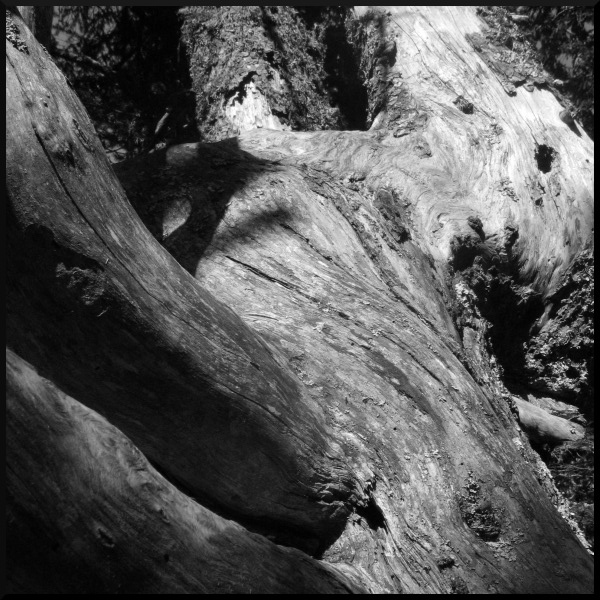
\includegraphics[width=8cm]{figures/tree04.jpg}
\caption{Árbol antiguo}
\end{figure}

\subsection{Inserción de órdenes de línea de comandos}

\begin{listing}[style=consola, numbers=none]
 gcc  -o e21 e21.c
\end{listing}





\subsection{Inserción de Código}

\begin{lstlisting}[caption=Ejemplo de código,style=C]

##include <stdio.h>
#include <sys/types.h>
#include <unistd.h>
#include <stdlib.h>

int main(void){

int register i;
int numHijos=4;
pid_t childpid;

for (i=0;i<numHijos;i++)
  if (childpid=fork()==0){
    sleep(1);
    printf("Proceso %ld con padre %ld\n", (long)getpid(), (long)getppid());
    exit(0);
  }

printf("Soy el proceso padre %ld\n", (long)getpid());
return 0;
}
\end{lstlisting}




\section{MEDIOS QUE SE PRETENDEN UTILIZAR}

\subsection{Medios Hardware}

El alumno deberá describir los medios hardware que prevé serán necesarios para el
desarrollo del proyecto.


\subsection{Medios Software}

El alumno deberá describir los medios software (lenguajes, entornos de desarrollo,
herramientas de gestión y planificación, etc.) que prevé serán necesarios para el
desarrollo del proyecto


\section{REFERENCIAS}

En esta sección se incluirán todas las referencias bibliográficas, ordenadas
alfabéticamente por el primer apellido del primer autor, de las obras de las cuales se
haya realizado alguna cita en los apartados anteriores. Las referencias deberán contener
datos básicos como nombre y apellidos de los autores, título de la obra, evento al que
pertenece, páginas, fecha y lugar de celebración (si se tratara de artículos de congreso),
ISBN, editorial y ciudad (si se tratara de libro), nombre de revista, páginas, volumen y
número (si se tratara de revista), etc.

Se empleará un formato de referencia reconocido en el ámbito académico como
ACM\footnote{http://www.acm.org/sigs/publications/proceedings-templates}\footnote{http://www.cs.ucy.ac.cy/\~{}chryssis/specs/ACM-refguide.pdf}.
Otros formatos aconsejables son, por ejemplo, IEEE, AMA, APA y AMA.

A continuación una sección de «Referencias» con ejemplos de referencias con formato ACM para:

\begin{itemize}
\item Un artículo de revista~\cite{Bow93}.
\item Un informe técnico~\cite{Ding97}.
\item Un libro~\cite{Tavel07}.
\item Un capítulo de libro~\cite{Greiner99}.
\item Un artículo en las actas de un congreso~\cite{Frohlic00}.
\item Para una página web~\cite{Steele04} (con autores conocidos).
\item Para una página web~\cite{Oxygen} (con autores desconocidos).
\end{itemize}


\bibliographystyle{alpha}
\singlespacing
\bibliography{ejemplo}


\end{document}


% Local Variables:
% coding: utf-8
% mode: flyspell
% ispell-local-dictionary: "castellano8"
% mode: latex
% End:
